\documentclass[12pt, titlepage]{article}

\usepackage{amsmath, mathtools}

\usepackage[round]{natbib}
\usepackage{amsfonts}
\usepackage{amssymb}
\usepackage{graphicx}
\usepackage{colortbl}
\usepackage{xr}
\usepackage{hyperref}
\usepackage{longtable}
\usepackage{xfrac}
\usepackage{tabularx}
\usepackage{float}
\usepackage{siunitx}
\usepackage{booktabs}
\usepackage{multirow}
\usepackage[section]{placeins}
\usepackage{caption}
\usepackage{fullpage}
\externaldocument{../../SRS/SRS} 
\externaldocument{../MG/MG}
\hypersetup{
bookmarks=true,     % show bookmarks bar?
colorlinks=true,       % false: boxed links; true: colored links
linkcolor=red,          % color of internal links (change box color with linkbordercolor)
citecolor=blue,      % color of links to bibliography
filecolor=magenta,  % color of file links
urlcolor=cyan          % color of external links
}

\usepackage{array}
\newcommand{\rref}[1]{R\ref{#1}}
\newcommand{\ddref}[1]{DD\ref{#1}}
\newcommand{\mref}[1]{M\ref{#1}}
\newcommand{\aref}[1]{A\ref{#1}}
%% Comments

\usepackage{color}

\newif\ifcomments\commentstrue

\ifcomments
\newcommand{\authornote}[3]{\textcolor{#1}{[#3 ---#2]}}
\newcommand{\todo}[1]{\textcolor{red}{[TODO: #1]}}
\else
\newcommand{\authornote}[3]{}
\newcommand{\todo}[1]{}
\fi

\newcommand{\wss}[1]{\authornote{blue}{SS}{#1}}
\newcommand{\an}[1]{\authornote{magenta}{Author}{#1}}


\newcommand{\progname}{Breaking Effect}

\begin{document}

\title{Module Interface Specification for Breaking Effect}

\author{Marshall Xiaoye Ma}

\date{\today}

\maketitle

\pagenumbering{roman}

\section{Revision History}

\begin{tabularx}{\textwidth}{p{3cm}p{2cm}X}
\toprule {\bf Date} & {\bf Version} & {\bf Notes}\\
\midrule
Date 2017-11-17 & 1.0 & New doc\\
\bottomrule
\end{tabularx}

~\newpage

\section{Symbols, Abbreviations and Acronyms}

See SRS Documentation at \url{https://github.com/MaXiaoye/cas741/blob/master/Doc/SRS/SRS.pdf}

\newpage

\tableofcontents

\newpage

\pagenumbering{arabic}

\section{Introduction}

The following document details the Module Interface Specifications for Breaking Effect. 
Breaking effect presents how the pieces of an object move after it separates into parts with
suddenness or violence.
\wss{It is usually a good idea to avoid one sentence paragraphs.}
\an{Merge the sentence into paragraph}
This project implements running time breaking effect in codes for 3-D models in unity3D without help from any similar plug-in. Including different shapes 3-D objects breaking based on physics and pieces interacting with the momentum provided by the breaking force. The breaking effect program simulates 3-D objects destruction process in vision by implementing scientific computing functions.

This project concentrates on calculation while
HCI or GUI are not important parts. Applied force is decided in codes in advance as input
and trace of motion is the output after calculation.

Complementary documents include the System Requirement Specifications
and Module Guide.  The full documentation and implementation can be
found at \url{https://github.com/MaXiaoye/cas741}.

\section{Notation}

The structure of the MIS for modules comes from \citet{HoffmanAndStrooper1995},
with the addition that template modules have been adapted from
\cite{GhezziEtAl2003}.  The mathematical notation comes from Chapter 3 of
\citet{HoffmanAndStrooper1995}.  For instance, the symbol := is used for a
multiple assignment statement and conditional rules follow the form $(c_1
\Rightarrow r_1 | c_2 \Rightarrow r_2 | ... | c_n \Rightarrow r_n )$.

The following table summarizes the primitive data types used by \progname. 

\begin{center}
\renewcommand{\arraystretch}{1.2}
\noindent 
\begin{tabular}{l l p{7.5cm}} 
\toprule 
\textbf{Data Type} & \textbf{Notation} & \textbf{Description}\\ 
\midrule
natural number & $\mathbb{N}$ & a number without a fractional component in [1, $\infty$) \\
real & $\mathbb{R}$ & any number in (-$\infty$, $\infty$)\\
String & String & represents sequences of characters.\\
Object & Object & A data structure to store attributes of input target object that provided by Unity3D. Defined in \mref{mTO}\\
PieceObject & PieceObj & A data structure to store attributes of pieces that generated as intermediate steps. It is defined in \mref{mPO}\\
\bottomrule
\end{tabular} 
\end{center}

\wss{As far as I can tell, you don't actually define Object or PieceObj anywhere.  You probably haven't done this because they are implemented elsewhere.  (I'm assuming they are implemented in Unit.)  However, you still need a spec of Object and PieceObj for your MIS to make sense.  You should create a simplified interface for these two ADTs.  You only need to document those parts that you actually need for your specification.}
\an{Sorry about the confusion ! Actually I define them in 2 modules. I add reference here.}

\noindent
The specification of \progname \ uses some derived data types: sequences, strings, and
tuples. Sequences are lists filled with elements of the same data type. Strings
are sequences of characters. Tuples contain a list of values, potentially of
different types. In addition, \progname \ uses functions, which
are defined by the data types of their inputs and outputs. Local functions are
described by giving their type signature followed by their specification.

\section{Module Decomposition}

The following table is taken directly from the Module Guide document for this project.

\begin{table}[h!]
	\centering
	\begin{tabular}{p{0.3\textwidth} p{0.6\textwidth}}
		\toprule
		\textbf{Level 1} & \textbf{Level 2}\\
		\midrule
		
		{Hardware-Hiding Module} & ~ \\
		\midrule
		
		\multirow{7}{0.3\textwidth}{Behaviour-Hiding Module} & Input module\\
		& Piece object module\\
		& Acquire pieces module\\
		& Displacement calculation module\\
		\midrule
		
		\multirow{3}{0.3\textwidth}{Software Decision Module} & Target object module\\
		& Collision with ground detection module\\
		& Output module\\
		& Camera controlling module\\
		\bottomrule
		
	\end{tabular}
	\caption{Module Hierarchy}
	\label{TblMH}
\end{table}

\begin{figure}[H]
	\centering
	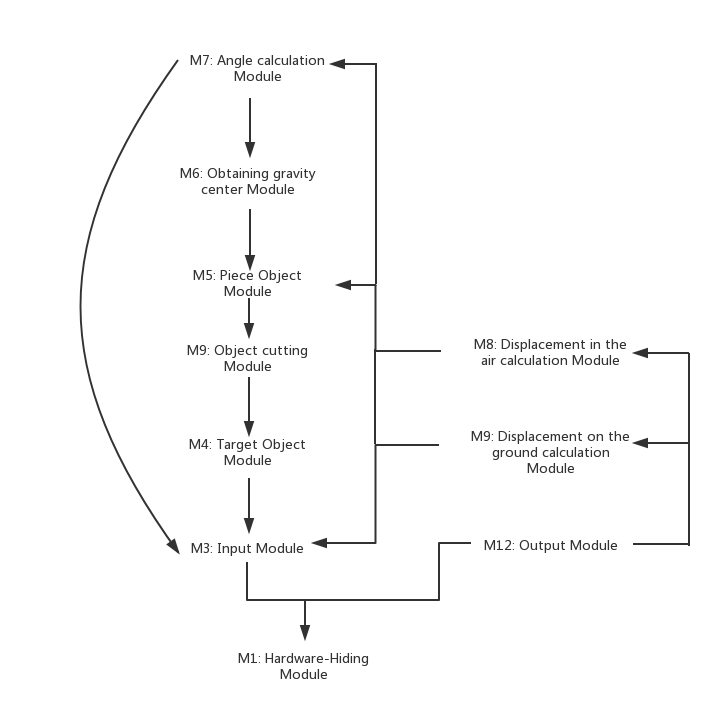
\includegraphics[width=1.1\textwidth]{./Figure1.png}
	\caption{Use hierarchy among modules}
	\label{FigUH}
\end{figure}

\wss{This figure is difficult to read.  You could make it bigger, or save it as
	+  a pdf, which avoids the rasterization of png.}
\an{Adjust size of figure}
~\newpage

\section{MIS of Input Module(\mref{mIF})} 
\label{Sec_MIM}

This module collect verifies input from user and store in corresponding variables. Include position of target object, explosion level, coefficient of ground friction.

\subsection{Module}

InputModule

\subsection{Uses}

Hardware-Hiding Module(\mref{mHH})\\
Target Object Module(\mref{mTO})(Section\ref{Sec_TOM})

\subsection{Syntax}

\subsubsection{Exported Access Programs}

\begin{center}
\begin{tabular}{p{3cm} p{4cm} p{4cm} p{2cm}}
\hline
\textbf{Name} & \textbf{In} & \textbf{Out} & \textbf{Exceptions} \\
\hline
InputVerify() &  $\mathbb{R}; \mathbb{R}; TargetObj$ & - & InvalidInput\\
\hline
\end{tabular}
\end{center}

\subsection{Semantics}

\subsubsection{Environment Variables}

\wss{This isn't how environment variables are used.  For a project like yours the only environment variables that would apply are external files and the screen.}
\wss{Why do you have TargetObj as both an environment variable and an input.  Ifit is an input, it isn't going to also appear as a state (or environment) variable.}
\an{I am wrong about how environment variables are used. I should not put variable in my class in environment part.}
\subsubsection{State Variables}

None

\subsubsection{Assumptions}

\begin{itemize}
	\item Object is a 3D model in Unity3D, which contains its position $(X,Y,Z)$
	\item The input target object must be splitted by external function that consists of sub-objects. Each sub-object will be considered and converted to a piece object in Breaking Effect. \wss{What does this mean?  If this is a Unity step, you should provide a pointer to an external resource that describes what this means.} \an{I change the description. Hope this makes it more clear.}
\end{itemize}
\subsubsection{Access Routine Semantics}

\noindent InputVerifiy($\mu_{k}$, E, $TargetObj$): \wss{The type in the syntax section does not match what is written here?  $\mathbb{R}^2$ means a sequence of two reals.  That means your syntax calls for two inputs, but you have 3. On the next page $\mu_k$ could be null.  null is not a float.} \an{Yeah $\mu_{k}$ and E don't form a sequence. I change the type in syntax section.}
\begin{itemize}
\item transition: N/A
\item output: Exceptions or None.
\item exception:\\
exc := ($\mu_{k}$ = null $\Rightarrow $ NoMuException)\\
exc := (E = null $\Rightarrow $ NoELvException)\\
exc := ($X \notin \mathbb{R} \vee (X \le -1000) \vee (X \ge 1000)$ $\Rightarrow $ InvalidCoorXException)\\
exc := ($Z \notin \mathbb{R} \vee (Z \le -1000) \vee (Z \ge 1000)$ $\Rightarrow $ InvalidCoorZException)\\
exc := ($Y != 0$ $\Rightarrow $ InvalidCoorYException)\\
exc := ($E \notin \mathbb{R} \vee (E \leq 0) \vee (E \geq 10)$ $\Rightarrow $ InvalidELvException)\\
exc := ($\mu_{k} \notin \mathbb{R} \vee (\mu_{k} \le 0) \vee (\mu_{k} \ge 1)$ $\Rightarrow $ InvalidMuException)\\
\end{itemize}

\section{MIS of piece object module(\mref{mPO})}
\label{Sec_POM}
Customize class for pieces. Pieces are generated after explosion happens to replace original target object from input.

\subsection{Module}

ObjCutModule

\subsection{Uses}

Input Module(\mref{mIF})(Section\ref{Sec_MIM})\\
Displacement calculation Module(\mref{mDC1})(Section\ref{Sec_DCM})\\ \wss{This reference did not work when I clicked on it.}

\subsection{Syntax}

\subsubsection{Exported Access Programs}

\begin{center}
	\begin{tabular}{p{4cm} p{4cm} p{4cm} p{2cm}}
		\hline
		\textbf{Name} & \textbf{In} & \textbf{Out} & \textbf{Exceptions} \\
		\hline		
		PieceObj() & $\mathbb{R}; \mathbb{R};Object$ & - & - \\
		MoveInAir() & - & - & - \\
		MoveOnGround() & - & - & - \\
		thetaOneCalc() & - & - & - \\
		thetaTwoCalc() & - & - & - \\
		Translate() & $\mathbb{R};\mathbb{R};\mathbb{R}$ & - & - \\
		\hline
	\end{tabular}
\end{center}

\wss{These don't look like access programs.  Isn't PieceObj a type?  If it is a constructor for PieceObj, then  you should document this in the MIS for the PieceObj ADT.} \an{PieceObj() is not a type but a constructor for PieceObj.}
\subsection{Semantics}

\subsubsection{Environment Variables}

\wss{Please review what environment variables are used for.}
\an{I put variable in my class in state variable section}
\subsubsection{State Variables}

$PieceObj.obj: Object$\\
$PieceObj.obj.transform.x: \mathbb{R}$\\
$PieceObj.obj.transform.y: \mathbb{R}$\\
$PieceObj.obj.transform.z: \mathbb{R}$\\
$PieceObj.onGround: Boolean$\\
$PieceObj.stop: Boolean$\\
$PieceObj.\theta_{1}: \mathbb{R}$\\
$PieceObj.\theta_{2}: \mathbb{R}$\\
$PieceObj.initSpeed: \mathbb{R}$\\
$PieceObj.speedThisFrameX: \mathbb{R}$\\
$PieceObj.speedLastFrameX: \mathbb{R}$\\
$PieceObj.speedThisFrameZ: \mathbb{R}$\\
$PieceObj.speedLastFrameZ: \mathbb{R}$

\subsubsection{Assumptions}

\noindent
\begin{itemize}
	\item obj is the 3D model of PieceObj in scene. 	
	\item $x,y,z$ are coordinates of object.	
	\item onGround indicates if the object is on the ground.	 
	\item $\theta_{1}$ is the angle between initial speed $v_{0}$ and horizontal.
	\item $\theta_{2}$ is the angle between $x$ axiom and projection on horizontal of initial speed
	\item initSpeed is the initial speed the object has when explosion happens.
	\item PieceObj() is constructor that use input from \mref{mIF}.
	\item Translate() controls motion of the object.
	\item  MoveInAir() and MoveOnGround() controls motion of the object by calling Translate(). It checks onGround firstly to make sure the object is in the air or on the ground. Based on value of bool variable onGround, that call and provide corresponding destination as input to Translate(). Destination to Translate() is calculated by \mref{mDC1}.
	\item Speed*Frame* values are used when calculate displacement on the ground for each piece. speedLastFrameX and speedLastFrameZ is the speed on X or Z direction at the beginning of last frame.
	speedThisFrameX and speedThisFrameZ is the speed on X or Z direction at the beginning of this frame. Unity considers negative speed as speed on opposite direction. So these 2 value are used to detect if speed of a piece reaches 0 by check if speedThisFrameX * speedLastFrameX $\leq$ 0. Then set stop to true.
	\item stop indicates if the speed of object already equals to 0.
\end{itemize}

\subsubsection{Access Routine Semantics}

\noindent PieceObj():
\begin{itemize}
	\item transition: Initialize PieceObj
	\item output: None
	\item exception: None
\end{itemize}

\noindent MoveInAir(): \an{use \mref{mDC1} here}
\begin{itemize}
	\item transition: Move PieceObj in the air by updating $x,y,z$
	\item output: None
	\item exception: None
\end{itemize}

\noindent MoveOnGround(): \an{use \mref{mDC1} here}
\begin{itemize}
	\item transition: Move PieceObj on the ground by updating $x,y,z$
	\item output: None
	\item exception: None
\end{itemize}

\subsubsection{Local functions}

\noindent thetaOneCalc(): \wss{This (and other access programs) do not appear in the syntax section.}\\ \an{Put thetaOneCalc() and thetaTwoCalc() to local function section}
Calculate the angle between initial speed $v_{0}$ and horizontal $\theta_{1}$. \an{$\theta_{1}$ and $\theta_{2}$ are values of each PieceObj}\\
Equation: $\theta_{1}=arctan \frac{y_{n} - Y}{\sqrt{(x_{n}-X)^2+(z_{n}-Z)^2}}$\\
%Convert equation to codes:Mathf.Atan(PieceObj.y / Mathf.Sqrt(Mathf.Pow(PieceObj.x - TargetObj.x,2) + Mathf.Pow(PieceObj.z - TargetObj.z,2))); 
\wss{Redefining the equation in code isn't usually done in the MIS.  If you instead defined a local function with parameters, and then in your spec called the local function with the parameters set to the code object variables, that would help explain how the parts of your implementation are connected.} \an{Yes ! follow the advice ! These 2 functions take no parameters because it can access its own variable inside object(by using pointer this.) and static variable.}
\begin{itemize}
	\item transition: $\theta_{1}: null \to \mathbb{R}$   
	\item output: None
	\item exception: None
\end{itemize}

\noindent thetaTwoCalc():\\
Calculate the angle between $x$ axiom and projection on horizontal of initial speed $\theta_{2}$.\\
Equation: $\theta_{2}=arctan \frac{x_{n}-X}{z_{n}-Z}$\\
%Convert equation to codes:Mathf.Atan2(PieceObj.x - TargetObj.x, PieceObj.z - TargetObj.z)
\begin{itemize}
	\item transition: $\theta_{2}: null \to \mathbb{R}$  
	\item output: None
	\item exception: None
\end{itemize}

\section{MIS of acquire pieces module (\mref{mOGC})} 
\label{Sec_MAP}
\subsection{Module}

PieceInitModule

\subsection{Uses}

Input Module(\mref{mIF})(Section\ref{Sec_MIM})\\
Piece Object Module(\mref{mPO})(Section\ref{Sec_POM})\\
target object module(\mref{mTO})(Section\ref{Sec_TOM})\\

\subsection{Syntax}

\subsubsection{Exported Access Programs}

\begin{center}
	\begin{tabular}{p{2cm} p{4cm} p{4cm} p{2cm}}
		\hline
		\textbf{Name} & \textbf{In} & \textbf{Out} & \textbf{Exceptions} \\
		\hline
		Start() & - & - & -\\
		GetExplosionPoint() & - & $\mathbb{R}^{3}$ & -\\
		PieceObj() & $\mathbb{R};\mathbb{R};Object$ & PieceObj & -\\
		\hline		
	\end{tabular}
\end{center}

\subsection{Semantics}

\subsubsection{Environment Variables}

None

\subsubsection{State Variables}

targetObj: Object\\
subObj[]: list of Object\\
pieceObj[]: list of Piece Object\\

\subsubsection{Assumptions}

\noindent
\begin{itemize}
	\item targetObj is the 3D model of target object in scene.
	\item subObj[] is a list of sub objects under target Object. Since all pieces make up the whole target object, all pieces object are considered as sub objects of the target object in Unity3D. We need to get all sub objects firstly and then use these sub objects to construct piece objects defined by myself.
	\item pieceObj[] is a list of piece objects defined by myself.
	\item PieceObj() is constructor of piece object that defined in \mref{mPO}. \an{use \mref{mPO} here.}
\end{itemize}

\subsubsection{Access Routine Semantics}

\noindent GetExplosionPoint():
Calculate position of explosionPoint that is bottom center of target object
\begin{itemize}
	\item transition: None
	\item output: $\mathbb{R}^{3}$
	\item exception: None
\end{itemize}

Do traversal to initialize all pieces. \an{Each piece is stored as an instance of class PieceObj defined in \mref{mPO}. Gravity center is position value in PieceObj}\\
targetObj = GameObject.Find("targetObj");\\
subObj = targetObj.GetComponentsInChildren<Transform>();\\
pieceObj = new PieceObj[targetObj.transform.childCount];\\
for (int i = 1; i < subObj.Length; i++) pieceObj[i - 1] = new PieceObj(subObj[i].gameObject, initSpeed, g);\\

\section{MIS of Displacement calculation module(\mref{mDC1})}
\label{Sec_DCM}
Calculate and output trace of motion for each piece in the air by using follow equations.
\subsection{Module}

DisAirCalModule

\subsection{Uses}

\subsection{Syntax}

\subsubsection{Exported Access Programs}

\begin{center}
	\begin{tabular}{p{3cm} p{6cm} p{4cm} p{2cm}}
		\hline
		\textbf{Name} & \textbf{In} & \textbf{Out} & \textbf{Exceptions} \\
		\hline
		DisAirCalX() & - & $\mathbb{R}$ & - \\
		DisAirCalY() & - & $\mathbb{R}$ & - \\
		DisAirCalZ() & - & $\mathbb{R}$ & - \\
		DisGroCalX() & - & $\mathbb{R}$ & - \\
		DisGroCalZ() & - & $\mathbb{R}$ & - \\
		\hline
	\end{tabular}
\end{center}

\subsection{Semantics}

\subsubsection{State Variables}

None

\subsubsection{Local constants}

FACTOR\_OF\_E: $\mathbb{R}$

\subsubsection{Access Routine Semantics}

\noindent DisAirCalX():\\
Equation: $v_{0}=$FACTOR\_OF\_E$*E ,S_{x}=v_{0}\cdot cos\theta _{1}\cdot sin\theta _{2}\cdot \Delta t$ \wss{Rather than hard code in the value 10, you should use a symbolic constant.}\an{Add it into local constants} \an{Based on \aref{A_velocity} \wss{This cross-reference didn't seem to work} in SRS that value of initial velocity given by explosion is ten times input $E$ unit length in unity per second. $\Delta t$ is the gap between each frame that input from unity3D} \an{Fixed!}\\
Convert equation to codes:\\
initSpeed * Mathf.Cos(PieceObj.theta1) * Mathf.Sin(PieceObj.theta2) * Time.deltaTime
\begin{itemize}
	\item transition: None
	\item output: $S_{x}: \mathbb{R}$ 
	\item exception: None
\end{itemize}

\noindent DisAirCalY():\\
Equation: $S_{y}=(v_{0}\cdot sin\theta _{1} - g \cdot t)\cdot \Delta t-\frac{1}{2}g \cdot \Delta t^{2}$
\an{t is real time since the explosion happens. So that $v_{0}\cdot sin\theta _{1} - g \cdot t$ means the initial speed on vertical direction at the beginning of each frame}\\
Convert equation to codes:\\
(initSpeed * Mathf.Sin(PieceObj.theta1) + g * Time.realtimeSinceStartup) * Time.deltaTime + 1 / 2 * g * Time.deltaTime * Time.deltaTime
\begin{itemize}
	\item transition: None
	\item output: $S_{y}: \mathbb{R}$ 
	\item exception: None
\end{itemize}

\noindent DisAirCalZ():\\
Equation:$S_{z}=v_{0}\cdot cos\theta _{1}\cdot cos\theta _{2}\cdot \Delta t$\\
Convert equation to codes:\\
initSpeed * Mathf.Cos(PieceObj.theta1) * Mathf.Cos(PieceObj.theta2) * Time.deltaTime)
\begin{itemize}
	\item transition: None
	\item output: $S_{z}: \mathbb{R}$ 
	\item exception: None
\end{itemize}

\noindent DisGroCalX():\\
Euqation: $a=\mu_{k}g$; $S_{x}=(v_{0}\cdot cos\theta _{1}\cdot sin\theta _{2} - at)\cdot \Delta t-\frac{1}{2}a \cdot \Delta t^{2}$\\
Convert equation to codes:\\
(initSpeed * Mathf.Sin(PieceObj.theta2) * Mathf.Cos(PieceObj.theta1) - a * Time.realtimeSinceStartup) * Time.deltaTime - 1 / 2 * a * Time.deltaTime * Time.deltaTime
\begin{itemize}
	\item transition: None
	\item output: $S_{x}: \mathbb{R}$ 
	\item exception: None 
\end{itemize}

\noindent DisGroCalZ():\\
Euqation: $a=\mu_{k}g$; $S_{z}=(v_{0}\cdot cos\theta _{1}\cdot cos\theta _{2} - at)\cdot \Delta t-\frac{1}{2}a \cdot \Delta t^{2}$\\
Convert equation to codes:\\
(initSpeed * Mathf.Cos(PieceObj.theta2) * Mathf.Cos(PieceObj.theta1) - a * Time.realtimeSinceStartup) * Time.deltaTime - 1 / 2 * a * Time.deltaTime * Time.deltaTime
\begin{itemize}
	\item transition: None
	\item output: $S_{z}: \mathbb{R}$ 
	\item exception: None 
\end{itemize}

\section{MIS of target object module(\mref{mTO})}
\label{Sec_TOM}
Object class provided by platform

\subsection{Module}

TarObjModule

\subsection{Uses}

\subsection{Syntax}

\subsubsection{Exported Access Programs}

\begin{center}
	\begin{tabular}{p{2cm} p{4cm} p{4cm} p{2cm}}
		\hline
		\textbf{Name} & \textbf{In} & \textbf{Out} & \textbf{Exceptions} \\
		\hline
		Find() & $String$ & Object & - \\
		\hline		
	\end{tabular}
\end{center}

\subsection{Semantics}

\subsubsection{Environment Variables}
None
\subsubsection{State Variables}

KeyCode.Space: Boolean.
This bool value indicates if key space is pressed on keyboard.\\
$TargetObj.transform.X: \mathbb{R}$\\
$TargetObj.transform.Y: \mathbb{R}$\\
$TargetObj.transform.Z: \mathbb{R}$

\subsubsection{Assumptions}

\noindent
\begin{itemize}
	\item $X,Y,Z$ are coordinates of object. Position is 3D vector that contains $X,Y,Z$ while it is also considered as gravity center location of the object
\end{itemize}

\subsubsection{Access Routine Semantics}

\noindent static Find($name: String$):
\begin{itemize}
	\item transition: Initialize an instance of target object by searching name.
	\item output: None
	\item exception: None
\end{itemize}


\section{MIS of Collision with ground detection Module (\mref{mOC})}
\label{Sec_CDM}
Detect if there is a collision between a piece and the ground. If so, set onGround
value to true.

\subsection{Module}

ColDetectModule

\subsection{Uses}

Piece Object Module(\mref{mPO})(Section\ref{Sec_POM})

\subsection{Syntax}

\subsubsection{Exported Access Programs}

\begin{center}
	\begin{tabular}{p{4cm} p{4cm} p{4cm} p{2cm}}
		\hline
		\textbf{Name} & \textbf{In} & \textbf{Out} & \textbf{Exceptions} \\
		\hline
		OnTriggerEnter() & - & - & - \\
		\hline
	\end{tabular}
\end{center}

\subsection{Semantics}

\subsubsection{Environment Variables}
None
\subsubsection{State Variables}

onGround

\subsubsection{Access Routine Semantics}

\noindent OnTriggerEnter():
\begin{itemize}
	\item transition: pieceObj.onGround: false $\to$ true;
	\item output: None 
	\item exception: None 
\end{itemize}

\section{MIS of Output Module(\mref{mOM})}
\label{Sec_MOM}
Unity3D interface with codes by calling function update() each frame. Unity3D convert data into visualization. Provide free camera for people to control view.

\subsection{Module}

OutputModule

\subsection{Uses}

Hardware-Hiding Module(\mref{mHH})\\
Piece Object Module(\mref{mPO})(Section\ref{Sec_POM})

\subsection{Syntax}

\subsubsection{Exported Access Programs}

\begin{center}
	\begin{tabular}{p{3cm} p{5cm} p{4cm} p{2cm}}
		\hline
		\textbf{Name} & \textbf{In} & \textbf{Out} & \textbf{Exceptions} \\
		\hline
		update() & codes to be run each frame & Visualization & - \\
		start() & - & - & - \\
		CameraControl & - & - & - \\
		\hline
	\end{tabular}
\end{center}

\subsection{Semantics}

\subsubsection{State Variables}
Scene
\subsubsection{Assumptions}

\noindent
\begin{itemize}
	\item Start is called on the frame when a script is enabled just before any of the Update methods is called the first time.
	\item Fixedupdate is called every frame. In Fixedupdate(), we listen if space is pressed as start point of the explosion. It also keeps updating status of all objects in the scene to convert location of objects to visualization that can be seen on the screen.
\end{itemize}

\subsubsection{Access Routine Semantics}

\noindent start():
\begin{itemize}
	\item transition: Initialization of scene.
	\item output: None 
	\item exception: None  
\end{itemize}

\noindent Fixedupdate():
\begin{itemize}
	\item transition: Piece objects $\rightarrow$ Visualization 
	\item output: None 
	\item exception: None  
\end{itemize}

\wss{You seem to be on the right track, but not following the MIS template makes the design difficult to review.  Please clarify your access programs, their input types, output types, your state variables, and your environment variables.}

\newpage

\bibliographystyle {plainnat}
\bibliography {../../../ReferenceMaterial/References}

\newpage

\end{document}
